%! Author = gramic
%! Date = 22.04.24

% Preamble
\begin{flushleft}
    \subsection{StackGres - Citus}
    \label{subsec:appendix_testing_stackgres_citus}
    Der Node ging down, als der Server \texttt{sks1184} heruntergefahren wurde:
    \begin{figure}[H]
        \centering
        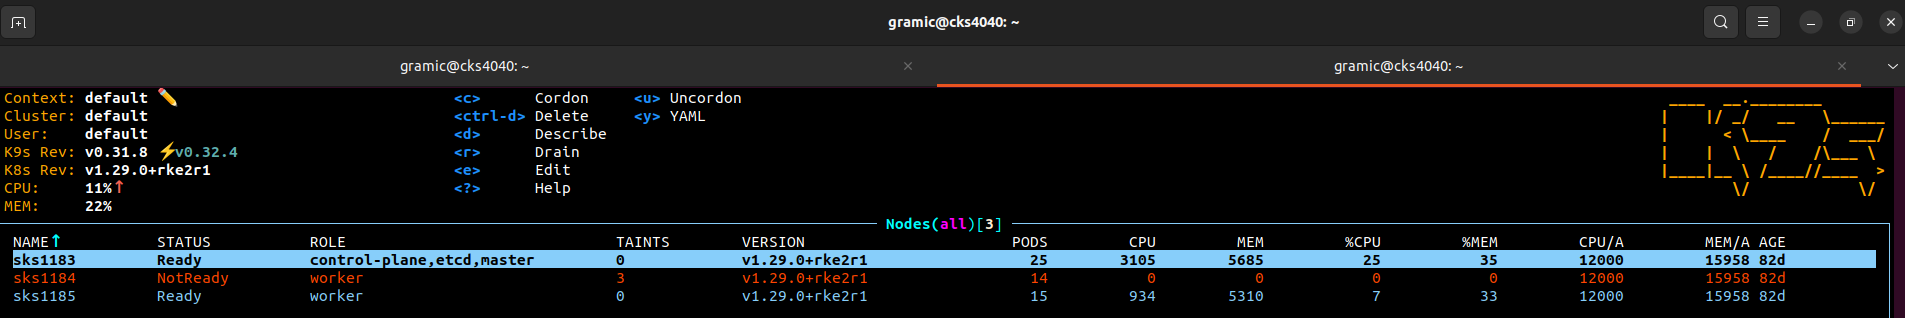
\includegraphics[width=0.5\linewidth]{source/appendix/evaluation_testing/stackgres_node_sks1184_down}
        \caption{StackGres Testing - Node sks1184 down}
        \label{fig:stackgres_node_sks1184_down}
    \end{figure}
    Entsprechend wurden die Pods ebenfalls auf \texttt{terminating} gesetzt:
    \begin{figure}[H]
        \centering
        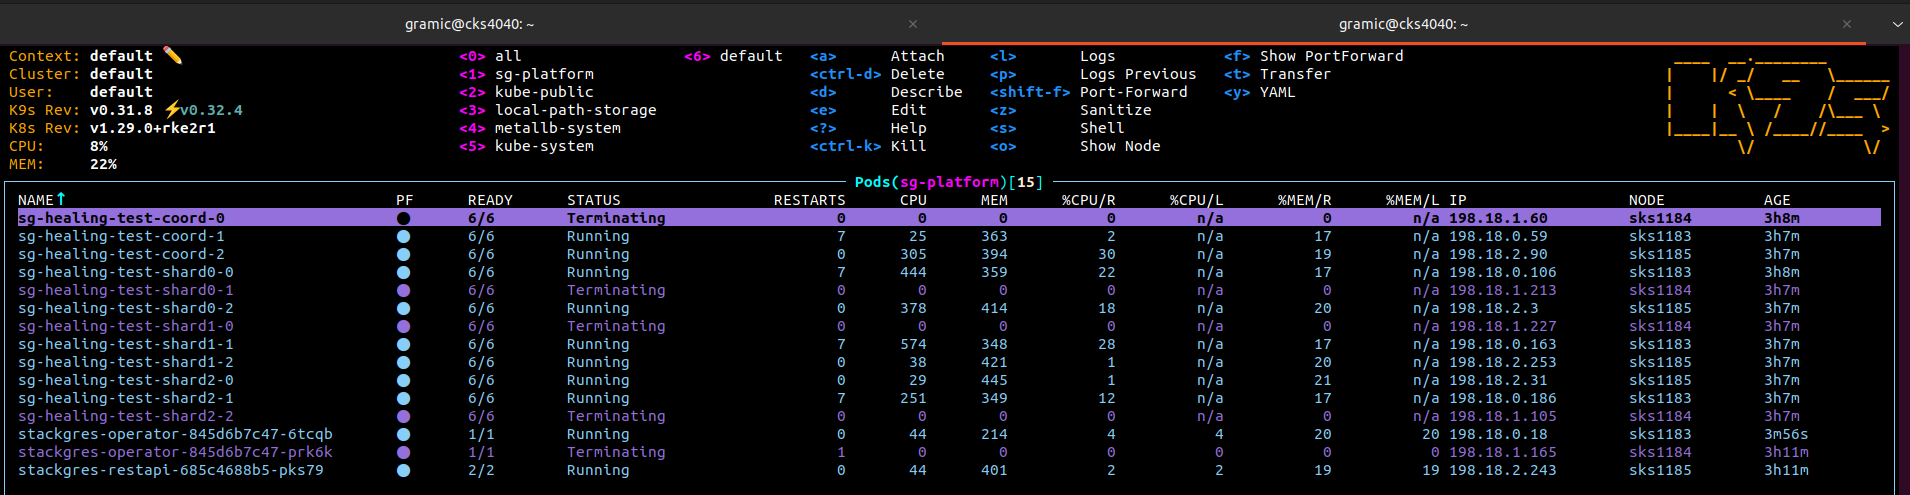
\includegraphics[width=1\linewidth]{source/appendix/evaluation_testing/stackgres_citus_testing_node_down}
        \caption{StackGres Testing - Pods Down}
        \label{fig:stackgres_citus_testing_node_down}
    \end{figure}
    Der Patroni-Leader des Coordinators aber auch die der Shards wurden einem \texttt{Failover} ausgeführt:
    \begin{figure}[H]
        \centering
        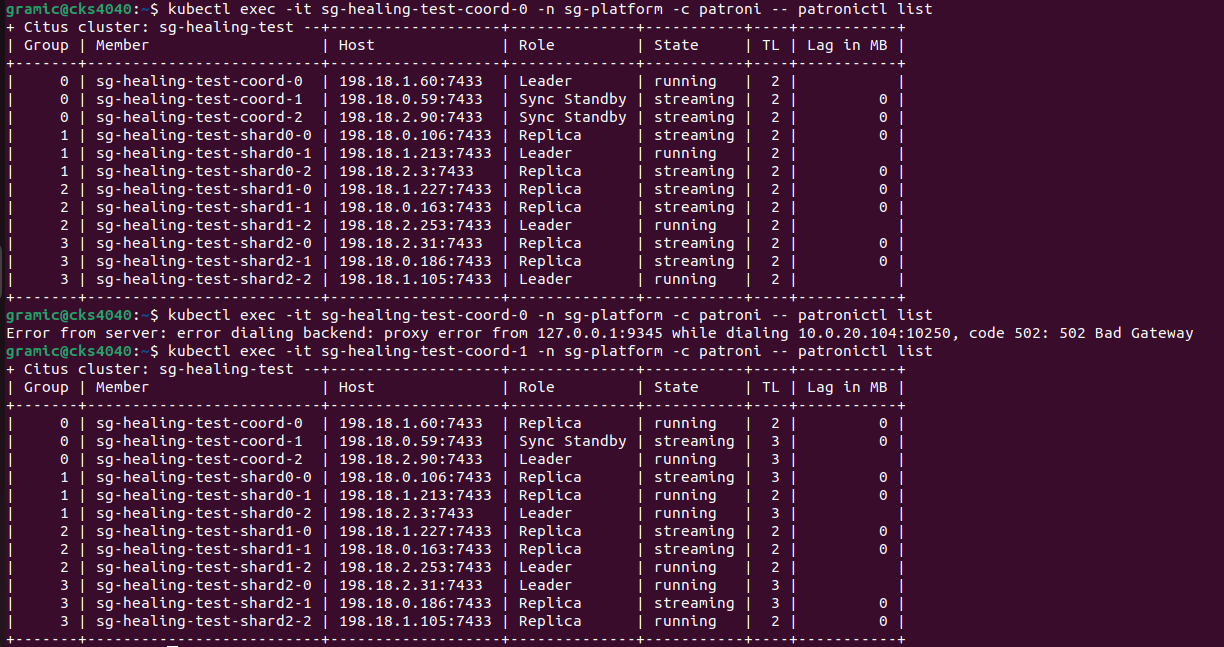
\includegraphics[width=1\linewidth]{source/appendix/evaluation_testing/stackgres_patroni_failover_overview}
        \caption{StackGres Testing - Patroni Übersicht}
        \label{fig:stackgres_patroni_failover_overview}
    \end{figure}
    Während dieser Zeit, ist die DB immer erreichbar:
    \begin{figure}[H]
        \centering
        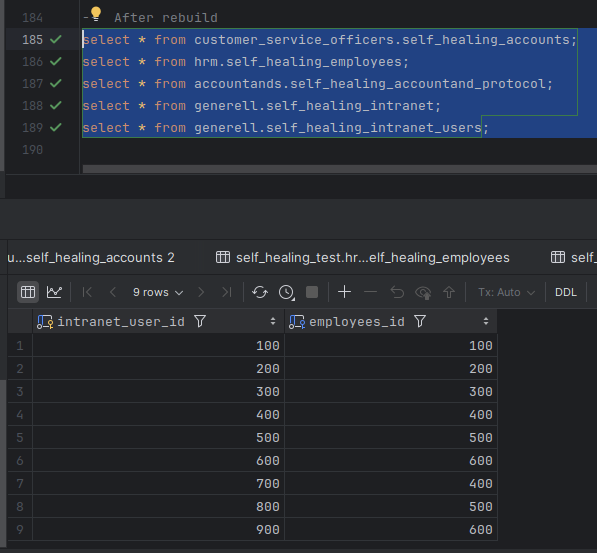
\includegraphics[width=1\linewidth]{source/appendix/evaluation_testing/stackgres_node_down_access_possible}
        \caption{StackGres Testing - DB Zugriff}
        \label{fig:stackgres_node_down_access_possible}
    \end{figure}
    Allerdings werden längere Transaktionen geschlossen:
    \begin{figure}[H]
        \centering
        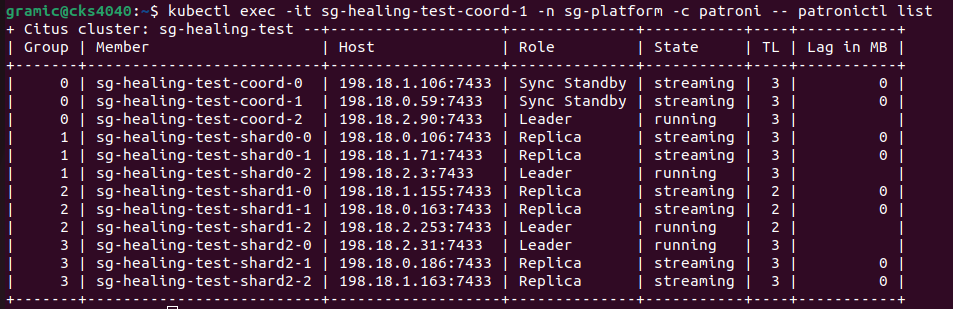
\includegraphics[width=1\linewidth]{source/appendix/evaluation_testing/stackgres_citus_connection_timeout}
        \caption{StackGres Testing - Connection Timeout}
        \label{fig:stackgres_citus_connection_timeout}
    \end{figure}
\end{flushleft}